
\section{Malloc routines}\label{sec:malloc}

Suppose that we are making a producer-consumer style program using PiP,
a PiP task is a producer and another PiP task is a consumer. Unlike the
conventional process model, there is no need of calling IPC (Inter
Process Communication) system call in PiP. All we have to do is just
passing pointers pointing data to be passed from the producer to the
consumer.

Here, an issue arises. If the passing data is allocated by a
\linuxfunc{malloc()} routine, then the passed data is
\linuxfunc{free()}ed by the consumer. As described so far, each PiP
task has its own \linuxfunc{malloc()} and \linuxfunc{free()} routines
associated with static variables holding and maintaining a memory
pool. The consumer receives 
the data allocated from the memory pool of the producer and tries to
\linuxfunc{free()} it when it becomes unnecessary. However, the
\linuxfunc{free()} routine on the consumer has no knowledge about the
producer-allocated memory region and fails
(Figure~\ref{fig:cross-malloc-free-issue}). I 
named this situation {\it cross-malloc-free}. 

\begin{figure}[ht]
\centering
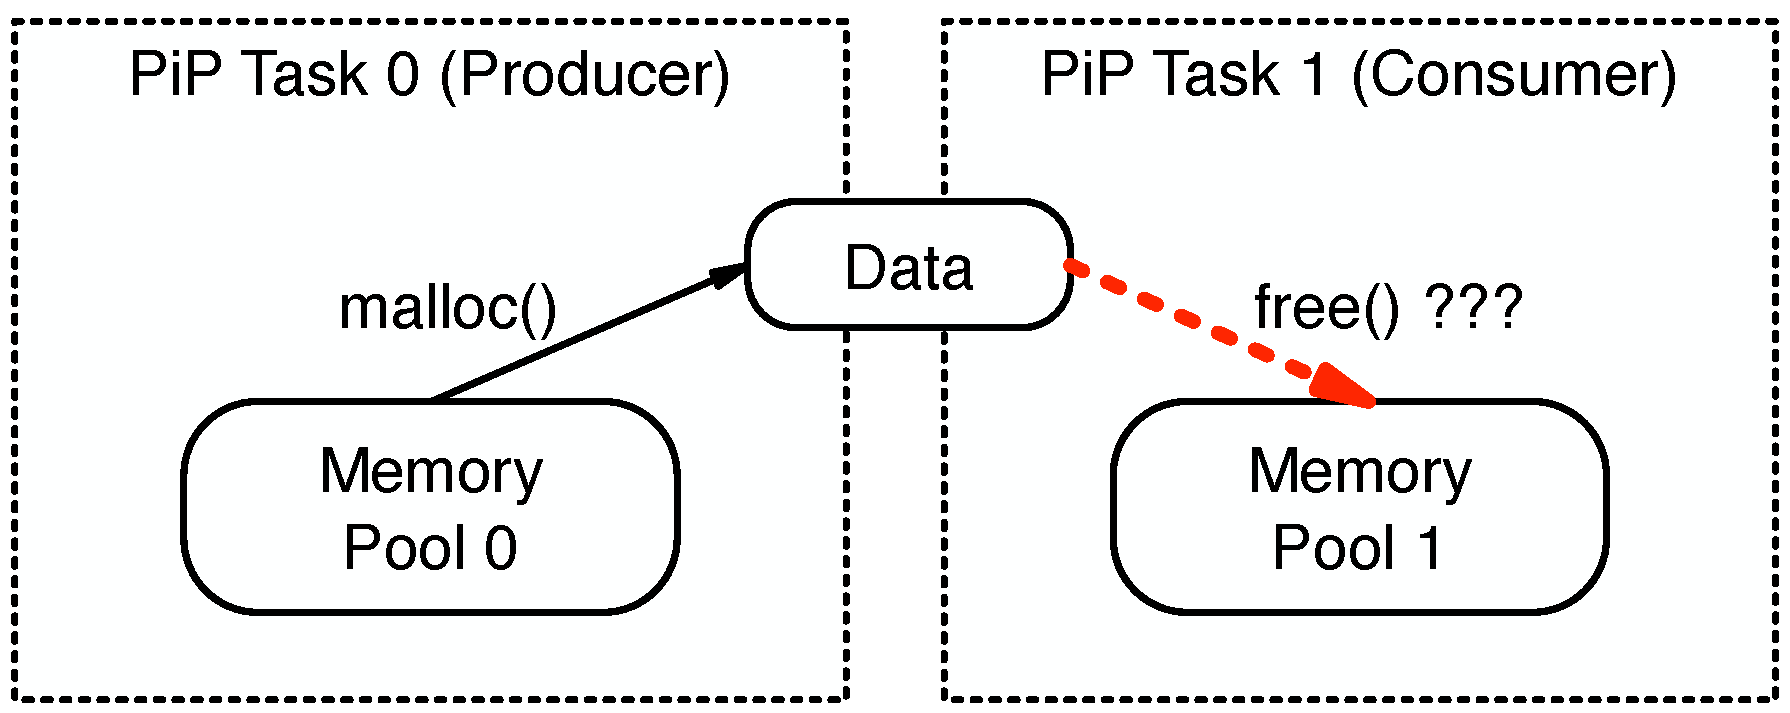
\includegraphics[width=0.7\columnwidth]{malloc/Figs/ProducerConsumer.pdf}
\caption{Cross-Malloc-Free Issue}
\label{fig:cross-malloc-free-issue}
\end{figure}

I tried this by using the \linuxfunc{malloc} routines provided Glibc and I
found that this works in most cases, not always. I do not know why
this works (again, {\bf in most cases}) with the Glibc \linuxfunc{malloc}
routines, but I believe this situation must be avoided.

\begin{figure}[ht]
\centering
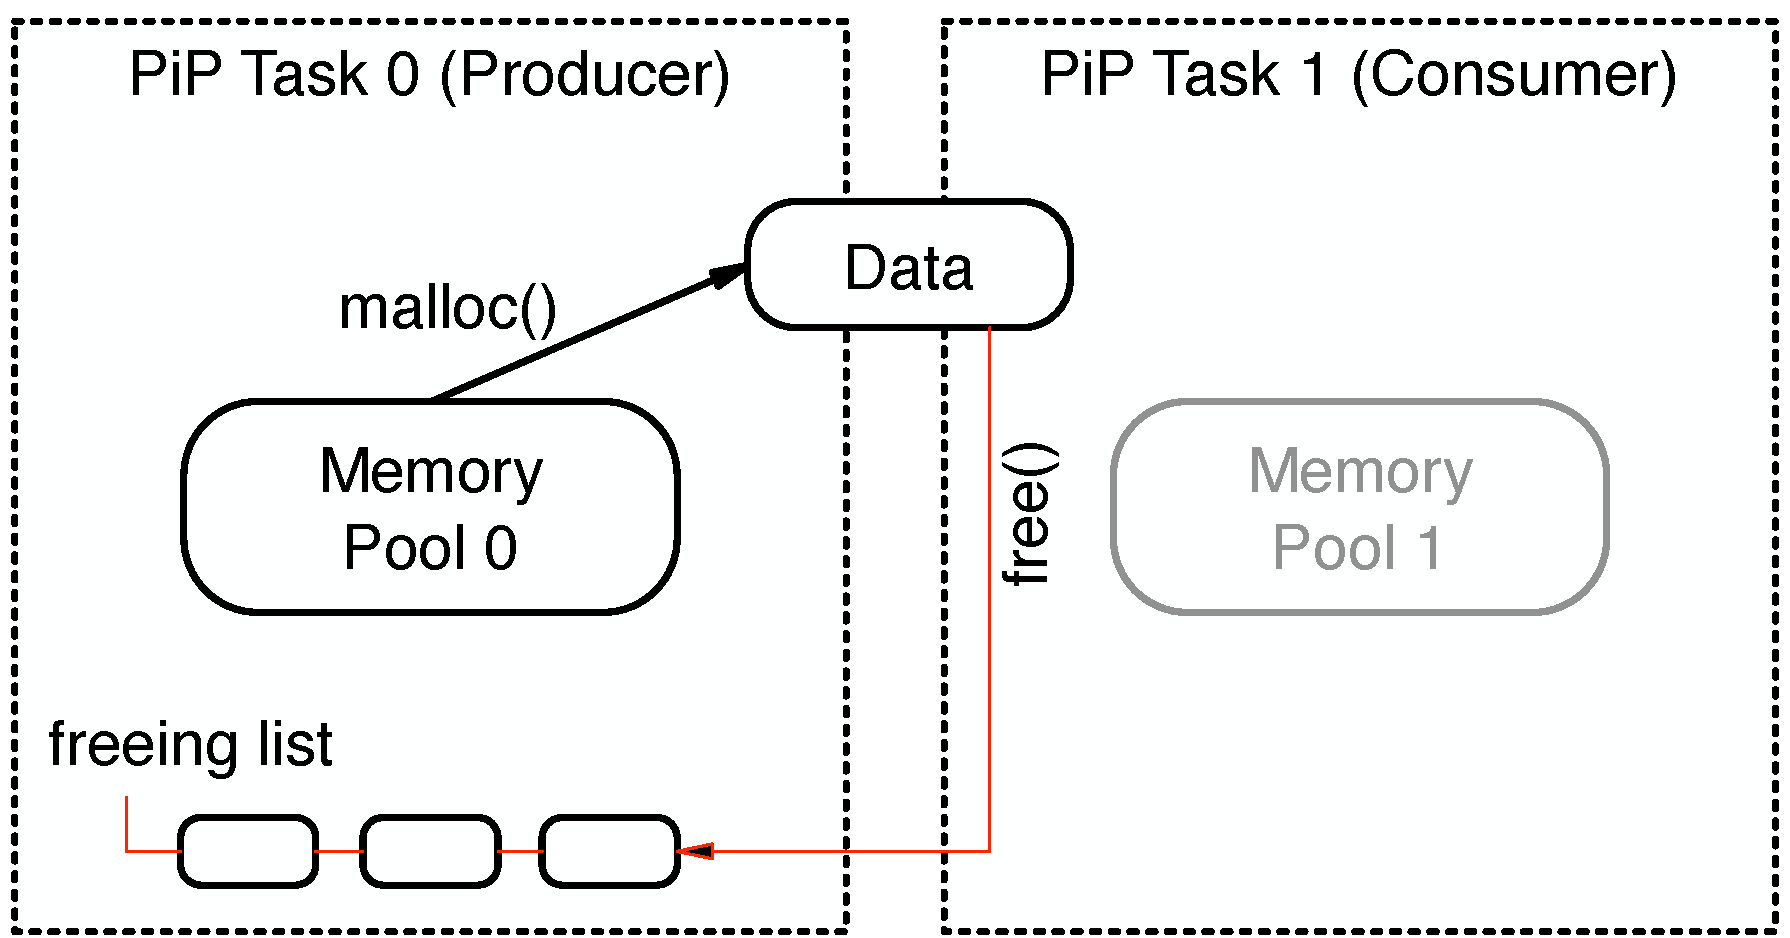
\includegraphics[width=0.7\columnwidth]{malloc/Figs/CrossMallocFree.pdf}
\caption{Cross-Malloc-Free with Freeing List}
\label{fig:cross-malloc-free}
\end{figure}

To deal with this, PiP library wraps \linuxfunc{malloc} routines as shown in
Table~\ref{tbl:pip-wrapper}. When a memory region is allocated, the
\linuxfunc{malloc} wrapper function embeds the information who
allocates that region. When this region is to be \linuxfunc{free()}ed, the
\linuxfunc{free()} wrapper function connects the region to the freeing
list of the task allocating the region. The regions in the freeing
list are eventually \linuxfunc{free()}ed when one of the \linuxfunc{malloc}
wrapper functions (Figure~\ref{fig:cross-malloc-free}).  
